\section{Machine Translation with Transformer}

\subsection*{Goal}

Translate a sentence from a source language to the target language. The problem is that there are many correct translations.

\subsection*{Seq2Seq Model}

Basically a representation method: $z=\encoder(x)$ and $y\mid x \sim \decoder(z)$.
We iteratively model $p(y_t\mid x, y_1, \dots, y_{t-1})$ because $p(y\mid x)=\prod_{t} p(y_t\mid x, y_1, \dots, y_{t-1})$.

At inference time, the model first predicts $y_1$ by $p(y_1\mid x)$, then $y_2$ by $p(y_2\mid x, y_1)$ and more.

For standard RNN, the decoder only receives one vector, causing information bottleneck.

\subsection*{Attention Mechanism}

\begin{center}
    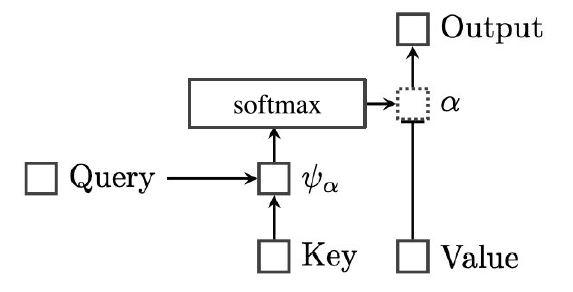
\includegraphics[width=.8\columnwidth]{img/attention.png}
\end{center}
Standard attention: what information from encoder is relevant for decoding step $t$. Use the output of encoder as key and value and the output of decoder at current step as the query.

Self-attention: what information from inputs are relevant for encoding step $t$ or what
information from (previous) outputs are relevant for decoding step $t$. Use only encoder's or decoder's output as key, query and value.